%=================================================================
% CSE 4345 — Big Data Analytics
% Week 5, Part 2: Seminal Research & Case Study
% Department of CSE, Premier University
%
% SEMINAL PAPER:
%   Vavilapalli et al. (2013) — Apache Hadoop YARN: Yet Another
%   Resource Negotiator. ACM SoCC 2013. (cited >3,000 times)
%
% CASE STUDY:
%   LinkedIn YARN Cluster (2013–2016) — Multi-Framework Big Data
%   Infrastructure at Professional-Network Scale
%=================================================================

\documentclass[aspectratio=169,10pt]{beamer}

%---------- Packages ----------
\usepackage[utf8]{inputenc}
\usepackage[T1]{fontenc}
\usepackage{booktabs}
\usepackage{xcolor}
\usepackage{tikz}
\usetikzlibrary{shapes.geometric, positioning, arrows.meta, decorations.pathreplacing}
\usepackage{amsmath}
\usepackage{graphicx}
\usepackage{multicol}
\usepackage{enumerate}
\usepackage{array}

%---------- Theme ----------
\usetheme{Madrid}

%---------- Premier University Color Identity ----------
\definecolor{PUNavy}{RGB}{10,36,99}
\definecolor{PUGold}{RGB}{197,151,37}
\definecolor{PULightBlue}{RGB}{210,228,255}
\definecolor{PUTeal}{RGB}{0,100,100}
\definecolor{PUGray}{RGB}{90,90,90}
\definecolor{PURed}{RGB}{160,30,30}
\definecolor{PUGreen}{RGB}{30,120,60}
\definecolor{PUPurple}{RGB}{90,30,120}
\definecolor{PUOrange}{RGB}{190,90,20}

\setbeamercolor{palette primary}{bg=PUNavy, fg=white}
\setbeamercolor{palette secondary}{bg=PUNavy!85, fg=white}
\setbeamercolor{palette tertiary}{bg=PUNavy!70, fg=white}
\setbeamercolor{palette quaternary}{bg=PUNavy, fg=white}
\setbeamercolor{structure}{fg=PUNavy}
\setbeamercolor{title}{bg=PUNavy, fg=PUGold}
\setbeamercolor{subtitle}{fg=white}
\setbeamercolor{frametitle}{bg=PUNavy, fg=PUGold}
\setbeamercolor{alerted text}{fg=PUGold!85!black}
\setbeamercolor{block title}{bg=PUNavy, fg=white}
\setbeamercolor{block body}{bg=PULightBlue!45}
\setbeamercolor{block title alerted}{bg=PUGold!80!black, fg=white}
\setbeamercolor{block body alerted}{bg=PUGold!12}
\setbeamercolor{block title example}{bg=PUTeal, fg=white}
\setbeamercolor{block body example}{bg=PUTeal!10}
\setbeamercolor{section in toc}{fg=PUNavy}
\setbeamercolor{itemize item}{fg=PUGold!80!black}
\setbeamercolor{itemize subitem}{fg=PUNavy!70}

\setbeamertemplate{navigation symbols}{}
\setbeamertemplate{itemize item}{\scriptsize\raise1.5pt\hbox{\textbullet}}
\setbeamertemplate{itemize subitem}{\scriptsize\raise1pt\hbox{--}}

%---------- Section separator ----------
\AtBeginSection[]{
  \begin{frame}[plain]
    \vfill
    \centering
    \begin{beamercolorbox}[sep=12pt,center,shadow=true,rounded=true]{block title}
      \usebeamerfont{title}\insertsectionhead\par
    \end{beamercolorbox}
    \vfill
  \end{frame}
}

%---------- Helper: citation box ----------
\newenvironment{paperbox}[1]{%
  \setbeamercolor{block title}{bg=PUNavy!90,fg=PUGold}
  \setbeamercolor{block body}{bg=PUNavy!6}
  \begin{block}{#1}}{%
  \end{block}}

%---------- Custom footline ----------
\setbeamertemplate{footline}{
  \leavevmode\hbox{%
    \begin{beamercolorbox}[wd=.333\paperwidth,ht=2.25ex,dp=1ex,center]{palette primary}
      \usebeamerfont{author in head/foot}\insertshortauthor
    \end{beamercolorbox}%
    \begin{beamercolorbox}[wd=.334\paperwidth,ht=2.25ex,dp=1ex,center]{palette secondary}
      \usebeamerfont{title in head/foot}\insertshorttitle
    \end{beamercolorbox}%
    \begin{beamercolorbox}[wd=.333\paperwidth,ht=2.25ex,dp=1ex,right]{palette primary}
      \usebeamerfont{date in head/foot}
      \insertframenumber{} / \inserttotalframenumber\hspace*{2ex}
    \end{beamercolorbox}}%
  \vskip0pt%
}

%---------- Title metadata ----------
\title[CSE 4345 \textbar{} Week 5, Part 2]{CSE 4345: Big Data Analytics}
\subtitle{Week 5, Part 2 \textemdash\ Seminal Research \& Case Study}
\author[Dept.\ of CSE]{Department of Computer Science \& Engineering\\[4pt]
       \small Premier University, Chittagong}
\institute{}
\date{Semester 2026}

%=================================================================
\begin{document}
%=================================================================

%----------------------------------------------------------------
% TITLE SLIDE
%----------------------------------------------------------------
\begin{frame}
  \titlepage
\end{frame}

%----------------------------------------------------------------
% PART 2 OVERVIEW
%----------------------------------------------------------------
\begin{frame}{Part 2 Overview — Week 5}
  \begin{columns}[T]
    \column{0.47\textwidth}
      \begin{block}{Today's Agenda}
        \tableofcontents
      \end{block}

    \column{0.50\textwidth}
      \begin{exampleblock}{Seminal Paper Covered}
        \begin{enumerate}
          \item Vavilapalli, V.~K., et al. (2013).
                \textit{Apache Hadoop YARN: Yet Another Resource
                Negotiator.} ACM SoCC 2013. Santa Clara, CA.
        \end{enumerate}
      \end{exampleblock}
      \vspace{6pt}
      \begin{alertblock}{Case Study}
        LinkedIn YARN Cluster (2013--2016): running MapReduce,
        Apache Spark, Apache Samza, and Apache Tez on a
        \textbf{single 5{,}000-node cluster}, processing
        500~TB/day for professional-network analytics.
      \end{alertblock}
      \vspace{4pt}
      \begin{block}{CLO Addressed}
        \textbf{CLO3} — Explain distributed resource management\\
        \textbf{PLO(b,c)}
      \end{block}
  \end{columns}
\end{frame}

%================================================================
\section{Research Paper — Vavilapalli et al.\ (2013): YARN}
%================================================================

%----------------------------------------------------------------
\begin{frame}{Research Landscape: Cluster Resource Management}
  \begin{center}
  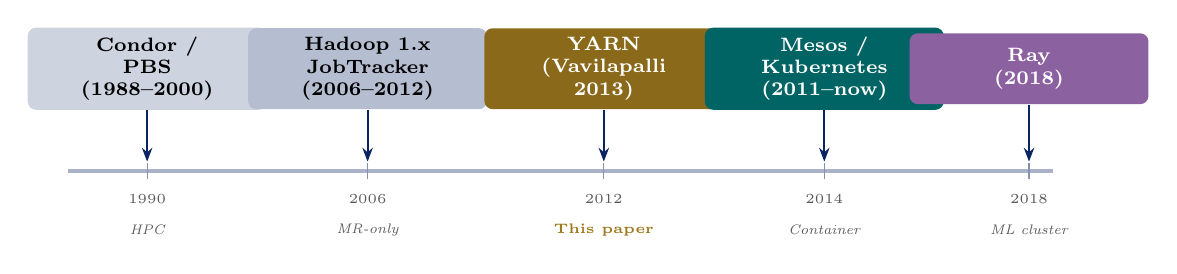
\begin{tikzpicture}[
      nbox/.style={rectangle, rounded corners=3pt, minimum width=3.0cm,
                   minimum height=0.9cm, text width=2.8cm, align=center,
                   font=\scriptsize\bfseries},
      arr/.style={-{Stealth[length=5pt]}, draw=PUNavy, thick}
    ]
    \draw[PUNavy!35, very thick] (0,0) -- (12.5,0);

    \node[nbox, fill=PUNavy!20]              (cond) at (1.0, 1.3)
          {Condor /\\PBS\\(1988--2000)};
    \node[nbox, fill=PUNavy!30]              (jt)   at (3.8, 1.3)
          {Hadoop 1.x\\JobTracker\\(2006--2012)};
    \node[nbox, fill=PUGold!70!black, text=white] (yarn) at (6.8, 1.3)
          {YARN\\(Vavilapalli\\2013)};
    \node[nbox, fill=PUTeal, text=white]     (mesos)at (9.6, 1.3)
          {Mesos /\\Kubernetes\\(2011--now)};
    \node[nbox, fill=PUPurple!70, text=white](ray)  at (12.2,1.3)
          {Ray\\(2018)};

    \foreach \x/\y in {1.0/1990, 3.8/2006, 6.8/2012, 9.6/2014, 12.2/2018}{
      \draw[PUNavy!50] (\x,0.1) -- (\x,-0.1);
      \node[font=\tiny, text=PUGray] at (\x,-0.35) {\y};
    }

    \draw[arr] (cond)  -- (1.0,  0.12);
    \draw[arr] (jt)    -- (3.8,  0.12);
    \draw[arr] (yarn)  -- (6.8,  0.12);
    \draw[arr] (mesos) -- (9.6,  0.12);
    \draw[arr] (ray)   -- (12.2, 0.12);

    \node[font=\tiny\itshape, text=PUGray]           at (1.0,  -0.75) {HPC};
    \node[font=\tiny\itshape, text=PUGray]           at (3.8,  -0.75) {MR-only};
    \node[font=\tiny\bfseries, text=PUGold!80!black] at (6.8,  -0.75) {This paper};
    \node[font=\tiny\itshape, text=PUGray]           at (9.6,  -0.75) {Container};
    \node[font=\tiny\itshape, text=PUGray]           at (12.2, -0.75) {ML cluster};
  \end{tikzpicture}
  \end{center}
  \vspace{4pt}
  \begin{alertblock}{The Core Problem YARN Solved}
    Hadoop 1.x's \textbf{JobTracker} mixed resource management and
    MapReduce-specific scheduling into a single process.
    This prevented any other framework (Spark, Tez, Samza) from running
    on the same cluster, and hit a hard scalability ceiling of
    $\approx$4{,}000 nodes.  YARN separated these concerns entirely.
  \end{alertblock}
\end{frame}

%----------------------------------------------------------------
\begin{frame}{Vavilapalli et al.\ (2013): Publication Context}
  \begin{columns}[T]
    \column{0.53\textwidth}
      \begin{paperbox}{Full Citation}
        Vavilapalli, V.~K., Murthy, A.~C., Douglas, C.,
        Agarwal, S., Konar, M., Evans, R., Graves, T.,
        Lowe, J., Shah, H., Seth, S., Saha, B., Curino, C.,
        O'Malley, O., Radia, S., Reed, B., \&
        Baldeschwieler, E. (2013).
        \textbf{Apache Hadoop YARN: Yet Another Resource Negotiator.}
        In \textit{Proc.\ 4th ACM Symposium on Cloud Computing
        (SoCC '13)}. Santa Clara, CA.\\[5pt]
        \textbf{Venue:} ACM SoCC — top cloud systems venue\\
        \textbf{Cited by:} $>$3{,}000 (Google Scholar, 2024)\\
        \textbf{Authors:} 16 engineers from Yahoo!, Hortonworks,
        and Microsoft — all active Hadoop committers
      \end{paperbox}
      \vspace{5pt}
      \begin{exampleblock}{Context: Why Now?}
        By 2012, Yahoo!\ ran 40{,}000-node clusters but a
        \emph{single} Hadoop~1.x JobTracker served all cluster traffic.
        Simultaneously, Apache Spark (2010) and Apache Tez (2013)
        needed a cluster resource manager — but could not use
        the MapReduce-specific JobTracker.
      \end{exampleblock}

    \column{0.44\textwidth}
      \begin{block}{The Hadoop 1.x Bottleneck}
        \begin{center}
        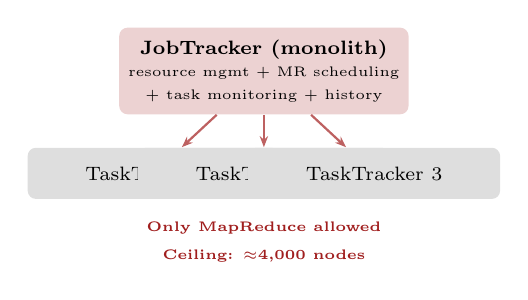
\begin{tikzpicture}[
            bx/.style={rectangle, rounded corners=3pt, minimum width=3.2cm,
                       minimum height=0.65cm, align=center, font=\scriptsize},
            arr/.style={-{Stealth[length=4pt]}, draw=PURed!70, thick}
          ]
          \node[bx, fill=PURed!20, minimum height=1.1cm, minimum width=3.6cm]
                (jt) at (0, 2.2)
                {\textbf{JobTracker (monolith)}\\
                 {\tiny resource mgmt + MR scheduling}\\
                 {\tiny + task monitoring + history}};
          \node[bx, fill=PUGray!20] (t1) at (-1.4, 0.9) {TaskTracker 1};
          \node[bx, fill=PUGray!20] (t2) at (0,    0.9) {TaskTracker 2};
          \node[bx, fill=PUGray!20] (t3) at (1.4,  0.9) {TaskTracker 3};
          \draw[arr] (jt) -- (t1);
          \draw[arr] (jt) -- (t2);
          \draw[arr] (jt) -- (t3);
          \node[font=\tiny\bfseries, text=PURed] at (0, 0.2)
                {Only MapReduce allowed};
          \node[font=\tiny\bfseries, text=PURed] at (0,-0.15)
                {Ceiling: $\approx$4{,}000 nodes};
        \end{tikzpicture}
        \end{center}
      \end{block}
  \end{columns}
\end{frame}

%----------------------------------------------------------------
\begin{frame}{Technical Contribution 1 — YARN Three-Layer Architecture}
  \begin{columns}[T]
    \column{0.46\textwidth}
      \begin{block}{The Three Layers}
        \textbf{1. ResourceManager (RM)} — one per cluster\\
        \begin{itemize}
          \item \textbf{Scheduler}: decides which application gets
                which containers; pluggable (FIFO, Capacity, Fair)
          \item \textbf{ApplicationsManager}: accepts job submissions,
                negotiates a container for each ApplicationMaster
        \end{itemize}
        \vspace{4pt}
        \textbf{2. NodeManager (NM)} — one per node\\
        \begin{itemize}
          \item Launches and monitors containers
          \item Reports CPU + memory usage to RM
          \item Manages local log aggregation
        \end{itemize}
        \vspace{4pt}
        \textbf{3. ApplicationMaster (AM)} — one per application\\
        \begin{itemize}
          \item Requests containers from RM
          \item Tells NMs to launch tasks inside containers
          \item Handles \emph{application-specific} fault tolerance
        \end{itemize}
      \end{block}

    \column{0.51\textwidth}
      \begin{center}
      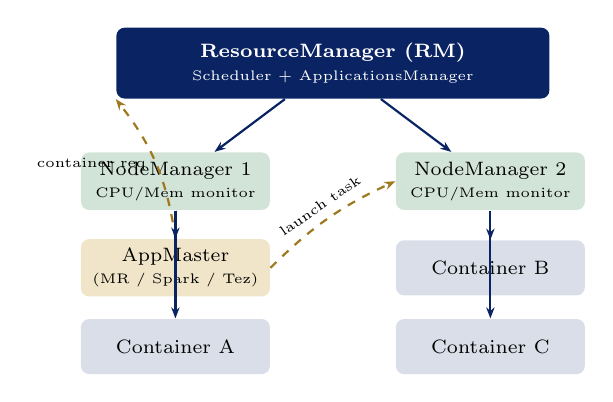
\begin{tikzpicture}[
          ybx/.style={rectangle, rounded corners=3pt, minimum width=3.0cm,
                      minimum height=0.7cm, align=center, font=\scriptsize},
          arr/.style={-{Stealth[length=4pt]}, draw=PUNavy, thick},
          darr/.style={-{Stealth[length=4pt]}, draw=PUGold!80!black,
                       thick, dashed}
        ]
        % RM
        \node[ybx, fill=PUNavy, text=white, minimum width=5.5cm,
              minimum height=0.9cm]
              (rm) at (0, 4.0)
              {\textbf{ResourceManager (RM)}\\
               {\tiny Scheduler + ApplicationsManager}};

        % Node 1
        \node[ybx, fill=PUGreen!20, minimum width=2.4cm]
              (nm1) at (-2.0, 2.5) {NodeManager 1\\{\tiny CPU/Mem monitor}};
        \node[ybx, fill=PUGold!25, minimum width=2.4cm]
              (am)  at (-2.0, 1.4) {AppMaster\\{\tiny (MR / Spark / Tez)}};
        \node[ybx, fill=PUNavy!15, minimum width=2.4cm]
              (c1)  at (-2.0, 0.4) {Container A};

        % Node 2
        \node[ybx, fill=PUGreen!20, minimum width=2.4cm]
              (nm2) at (2.0, 2.5) {NodeManager 2\\{\tiny CPU/Mem monitor}};
        \node[ybx, fill=PUNavy!15, minimum width=2.4cm]
              (c2)  at (2.0, 1.4) {Container B};
        \node[ybx, fill=PUNavy!15, minimum width=2.4cm]
              (c3)  at (2.0, 0.4) {Container C};

        % RM <-> NMs (resource reports)
        \draw[arr]  (rm)  -- (nm1);
        \draw[arr]  (rm)  -- (nm2);
        % AM negotiates with RM
        \draw[darr] (am.north) to[bend right=15]
              node[font=\tiny, left] {container req} (rm.south west);
        % AM instructs NM2
        \draw[darr] (am.east) to[bend left=10]
              node[font=\tiny, above, sloped] {launch task} (nm2.west);
        % NMs manage containers
        \draw[arr]  (nm1) -- (am);
        \draw[arr]  (nm1) -- (c1);
        \draw[arr]  (nm2) -- (c2);
        \draw[arr]  (nm2) -- (c3);
      \end{tikzpicture}
      \end{center}
  \end{columns}
\end{frame}

%----------------------------------------------------------------
\begin{frame}{Technical Contribution 2 — Container Model \& Schedulers}
  \begin{columns}[T]
    \column{0.50\textwidth}
      \begin{block}{Container: The Resource Unit}
        A \textbf{Container} is a bundle of resources on a specific node:
        \begin{itemize}
          \item \texttt{\{vcores: N, memory: M\,MB\}}
          \item The AM requests containers with specific resource
                requirements; the Scheduler decides which node to
                assign each container to
          \item Containers are \textbf{isolated} via Linux cgroups
                (CPU) and memory limits enforced by the NM
          \item If a container exceeds its memory limit, the NM
                \textbf{kills it immediately} to protect other containers
        \end{itemize}
      \end{block}
      \vspace{5pt}
      \begin{exampleblock}{Multi-Framework Enablement}
        Because the AM is \emph{per-application} and handles
        framework-specific logic, YARN is framework-agnostic.
        The same cluster runs:\\
        MapReduce AM $\;\bullet\;$ Spark AM $\;\bullet\;$
        Tez AM $\;\bullet\;$ Samza AM
      \end{exampleblock}

    \column{0.47\textwidth}
      \begin{block}{YARN Schedulers (Pluggable)}
        \renewcommand{\arraystretch}{1.25}
        \begin{tabular}{@{}lp{4.5cm}@{}}
          \toprule
          \textbf{Scheduler} & \textbf{Policy} \\
          \midrule
          FIFO        & One queue; first-come first-served.
                        Simple but starves long jobs. \\
          Capacity    & Multiple queues with capacity
                        guarantees; excess capacity shared.
                        Used by Yahoo!, LinkedIn. \\
          Fair        & Jobs share resources equally;
                        small jobs get fast turnaround.
                        Used by Facebook, Twitter. \\
          \bottomrule
        \end{tabular}
      \end{block}
      \vspace{5pt}
      \begin{alertblock}{Scalability Result (from the paper)}
        YARN was tested on a \textbf{6{,}000-node} cluster with
        \textbf{100{,}000 tasks} running simultaneously —
        exceeding Hadoop~1.x's~4{,}000-node limit by 50\%.
        The paper reports RM handling \textbf{1{,}000 heartbeats/sec}
        with $<$1~second scheduling latency.
      \end{alertblock}
  \end{columns}
\end{frame}

%----------------------------------------------------------------
\begin{frame}{Technical Contribution 3 — Fault Tolerance \& Timeline Server}
  \begin{columns}[T]
    \column{0.52\textwidth}
      \begin{block}{Layered Fault Tolerance in YARN}
        YARN delegates fault handling to three layers:
        \begin{enumerate}
          \item \textbf{NodeManager failure}: RM detects missing
                heartbeat ($>$10 min) and marks all containers on
                that node as failed.  The AM is notified and
                re-requests containers elsewhere.
          \item \textbf{ApplicationMaster failure}: RM restarts the AM
                (up to a configured max attempts, default~2).
                The new AM can recover job state from HDFS
                checkpoints if the framework supports it
                (MapReduce: yes; early Spark: no).
          \item \textbf{ResourceManager failure}: YARN~2.4+ added
                \textbf{RM High Availability} via ZooKeeper —
                an Active RM and a Standby RM; automatic failover
                in $<$60 seconds.
        \end{enumerate}
      \end{block}

    \column{0.45\textwidth}
      \begin{block}{Timeline Server: Observability}
        The \textbf{Application Timeline Server} (ATS) is a
        YARN component introduced alongside YARN:
        \begin{itemize}
          \item Stores per-application and per-container event history
          \item Accessible via REST API after job completion
          \item Powers the \textbf{YARN ResourceManager UI}
                (http://rm-host:8088)
          \item Enables post-mortem debugging:
                why did container C0001 fail? when did each task start?
        \end{itemize}
      \end{block}
      \vspace{5pt}
      \begin{exampleblock}{Hadoop 1 vs.\ YARN Comparison}
        \renewcommand{\arraystretch}{1.2}
        \scriptsize
        \begin{tabular}{@{}lcc@{}}
          \toprule
          & \textbf{Hadoop 1} & \textbf{YARN} \\
          \midrule
          Max nodes     & $\sim$4{,}000 & $>$10{,}000 \\
          Frameworks    & MR only       & Any (Spark, Tez \ldots) \\
          Resource unit & Slot (fixed)  & Container (flexible) \\
          AM            & In JobTracker & Per-app process \\
          RM HA         & No            & Yes (ZooKeeper) \\
          \bottomrule
        \end{tabular}
      \end{exampleblock}
  \end{columns}
\end{frame}

%----------------------------------------------------------------
\begin{frame}{Impact Today — Vavilapalli et al.\ (2013)}
  \begin{columns}[T]
    \column{0.50\textwidth}
      \begin{block}{YARN's Lasting Influence}
        \begin{itemize}
          \item \textbf{Apache Spark on YARN} (2013+): Spark's default
                cluster mode in enterprise Hadoop; YARN manages executor
                containers while Spark's AM handles DAG scheduling
          \item \textbf{Apache Tez} (2013): DAG-based successor to
                MapReduce; Hive and Pig rewrote execution engines to
                use Tez on YARN, reducing latency by $5\text{--}10\times$
          \item \textbf{Apache Samza} (LinkedIn, 2013): stream processing
                framework designed natively for YARN containers
          \item \textbf{YARN vs.\ Kubernetes} (2018--present):
                Kubernetes has largely replaced YARN for new deployments;
                but the \emph{three-tier design} (global scheduler /
                node agent / per-app master) is identical
          \item \textbf{AWS EMR, Azure HDInsight, Cloudera CDP}:
                all shipped YARN as the cluster OS through 2020
        \end{itemize}
      \end{block}

    \column{0.47\textwidth}
      \begin{exampleblock}{CMU 15-721 / Harvard CS265 Perspective}
        \begin{itemize}
          \item CMU 15-721 frames YARN's Scheduler as a
                \textbf{multi-resource bin-packing problem}:
                fitting $\{$vCPU, RAM$\}$ containers into
                heterogeneous nodes is NP-hard; YARN uses
                \emph{dominant resource fairness} (DRF)
          \item Harvard CS265 compares YARN's ApplicationMaster
                model to \textbf{Mesos's executor model}:
                YARN pushes scheduling intelligence into the AM
                (two-level scheduling), Mesos offers resource
                offers directly to frameworks (offer-based)
        \end{itemize}
      \end{exampleblock}
      \vspace{5pt}
      \begin{alertblock}{CLO3 Connection}
        YARN operationalises \textbf{CLO3} directly:
        explaining how distributed frameworks negotiate,
        isolate, and recover cluster resources at scale.
      \end{alertblock}
  \end{columns}
\end{frame}

%================================================================
\section{Case Study — LinkedIn YARN Cluster (2013--2016)}
%================================================================

%----------------------------------------------------------------
\begin{frame}{LinkedIn's Data Challenge}
  \begin{columns}[T]
    \column{0.52\textwidth}
      \begin{block}{Why LinkedIn Needed YARN Urgently}
        LinkedIn (acquired by Microsoft in 2016) ran the world's
        largest professional network, generating:
        \begin{itemize}
          \item \textbf{Profile views, connection requests, job searches}:
                $\approx$2 billion page-views/day by 2013
          \item \textbf{People You May Know (PYMK)}: graph algorithm
                over 300 million member profiles updated daily
          \item \textbf{Skills \& Endorsements}: collaborative filtering
                over 25 billion endorsement events
          \item \textbf{Ad targeting}: real-time bidding backed by
                offline feature engineering on member activity logs
          \item \textbf{Feed ranking}: news-feed ML models retrained
                every 4 hours on the latest engagement signals
        \end{itemize}
        All of these needed \textbf{different frameworks}: graph
        (Spark GraphX), stream (Samza), batch SQL (Hive), ML (Spark MLlib).
      \end{block}

    \column{0.45\textwidth}
      \begin{alertblock}{The Hadoop 1.x Wall}
        LinkedIn ran \textbf{separate clusters} per workload:
        \begin{itemize}
          \item \textbf{Cluster A}: MapReduce for Hive ETL
          \item \textbf{Cluster B}: experimental Spark cluster
          \item \textbf{Cluster C}: Samza stream processing nodes
        \end{itemize}
        Each cluster was \textbf{under-utilised} at different times.
        Cross-cluster data movement added latency.
        Managing three separate cluster configurations tripled ops cost.\\[6pt]
        YARN promised to \textbf{collapse all three into one}
        with fair resource sharing and framework isolation.
      \end{alertblock}
  \end{columns}
\end{frame}

%----------------------------------------------------------------
\begin{frame}{LinkedIn's Multi-Framework YARN Architecture}
  \begin{columns}[T]
    \column{0.50\textwidth}
      \begin{block}{Unified Cluster Design (2013--2016)}
        \begin{itemize}
          \item \textbf{Single 5{,}000-node YARN cluster}
                (Capacity Scheduler with 6 queues)
          \item \textbf{Queue allocation}:
                \begin{itemize}
                  \item \texttt{production} (40\%): Hive ETL, Pig
                  \item \texttt{spark} (25\%): Spark batch + MLlib
                  \item \texttt{samza} (15\%): Kafka consumer streams
                  \item \texttt{adhoc} (10\%): analyst Hive queries
                  \item \texttt{tez} (7\%): interactive Hive-on-Tez
                  \item \texttt{reserve} (3\%): overflow / burst
                \end{itemize}
          \item \textbf{Pre-emption enabled}: idle capacity in one
                queue borrowed by others; reclaimed with 30-second warning
          \item \textbf{Azkaban} (LinkedIn's open-source workflow
                scheduler) orchestrates cross-queue job pipelines
        \end{itemize}
      \end{block}

    \column{0.47\textwidth}
      \begin{center}
      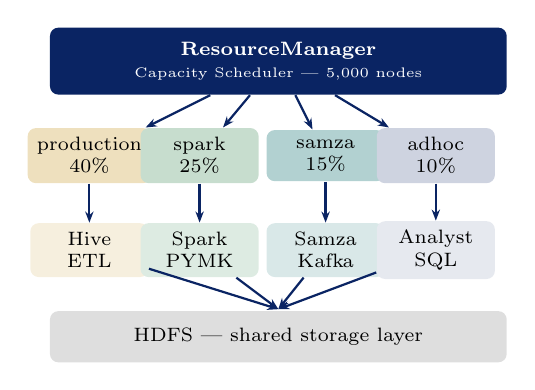
\begin{tikzpicture}[
          qbx/.style={rectangle, rounded corners=3pt, minimum width=1.5cm,
                      minimum height=0.65cm, align=center, font=\scriptsize},
          arr/.style={-{Stealth[length=4pt]}, draw=PUNavy, thick}
        ]
        \node[qbx, fill=PUNavy, text=white, minimum width=5.8cm,
              minimum height=0.85cm]
              (rm) at (0, 4.0)
              {\textbf{ResourceManager}\\{\tiny Capacity Scheduler — 5,000 nodes}};

        \node[qbx, fill=PUGold!30]   (q1) at (-2.4, 2.8) {production\\40\%};
        \node[qbx, fill=PUGreen!25]  (q2) at (-1.0, 2.8) {spark\\25\%};
        \node[qbx, fill=PUTeal!30]   (q3) at (0.6,  2.8) {samza\\15\%};
        \node[qbx, fill=PUNavy!20]   (q4) at (2.0,  2.8) {adhoc\\10\%};

        \foreach \q in {q1, q2, q3, q4} {
          \draw[arr] (rm) -- (\q);
        }

        \node[qbx, fill=PUGold!15]   (hive) at (-2.4, 1.6) {Hive\\ETL};
        \node[qbx, fill=PUGreen!15]  (sp)   at (-1.0, 1.6) {Spark\\PYMK};
        \node[qbx, fill=PUTeal!15]   (sam)  at (0.6,  1.6) {Samza\\Kafka};
        \node[qbx, fill=PUNavy!10]   (adq)  at (2.0,  1.6) {Analyst\\SQL};

        \draw[arr] (q1) -- (hive);
        \draw[arr] (q2) -- (sp);
        \draw[arr] (q3) -- (sam);
        \draw[arr] (q4) -- (adq);

        \node[qbx, fill=PUGray!20, minimum width=5.8cm]
              (hdfs) at (0, 0.5) {HDFS — shared storage layer};
        \foreach \n in {hive, sp, sam, adq} {
          \draw[arr] (\n) -- (0, 0.85);
        }
      \end{tikzpicture}
      \end{center}
  \end{columns}
\end{frame}

%----------------------------------------------------------------
\begin{frame}{Scale Numbers \& PYMK at LinkedIn}
  \begin{columns}[T]
    \column{0.52\textwidth}
      \begin{block}{LinkedIn YARN Cluster Scale (2015)}
        \renewcommand{\arraystretch}{1.3}
        \begin{tabular}{@{}ll@{}}
          \toprule
          \textbf{Metric}             & \textbf{Value} \\
          \midrule
          YARN cluster size           & 5{,}000 nodes \\
          Daily data processed        & 500 TB \\
          Peak containers running     & 400{,}000 \\
          Daily jobs submitted        & 30{,}000+ \\
          PYMK Spark job size         & 300M member graph \\
          PYMK recompute time (YARN)  & 4 hours (was 18 hr on MR1) \\
          Hive queries/day (analysts) & 8{,}000+ \\
          Samza Kafka lag (p99)       & $<$500 ms \\
          YARN cluster utilisation    & 78\% (vs.\ 45\% on 3 silos) \\
          \bottomrule
        \end{tabular}
      \end{block}

    \column{0.45\textwidth}
      \begin{exampleblock}{People You May Know (PYMK) Pipeline}
        PYMK is LinkedIn's friend-recommendation feature.
        Its batch pipeline on YARN:
        \begin{enumerate}\setlength\itemsep{2pt}
          \item \textbf{Ingest} (Samza): Kafka consumer reads
                member-profile-view events in real time
          \item \textbf{Feature store} (Hive): nightly ETL joins
                1st, 2nd, 3rd-degree connections for all 300M members
          \item \textbf{Graph model} (Spark GraphX): runs
                \textbf{label propagation} over the social graph
                to score $\approx$10B candidate pairs
          \item \textbf{Serve}: top-$k$ recommendations per member
                written to \textbf{Voldemort} (key-value store)
        \end{enumerate}
        All four steps share containers on the same YARN cluster.
      \end{exampleblock}
  \end{columns}
\end{frame}

%----------------------------------------------------------------
\begin{frame}{Lessons Learned \& Discussion Questions}
  \begin{columns}[T]
    \column{0.52\textwidth}
      \begin{block}{Key Lessons from LinkedIn's YARN Deployment}
        \begin{enumerate}
          \item \textbf{Resource consolidation increases utilisation}:
                merging 3 siloed clusters into one raised average
                utilisation from 45\% to 78\%
                — the same capacity served 73\% more workload
          \item \textbf{Capacity Scheduler enables SLAs}:
                production queues guaranteed minimum resources;
                analyst \texttt{adhoc} queries cannot starve
                revenue-generating pipelines
          \item \textbf{Pre-emption needs tuning}: aggressive
                pre-emption killed long-running Spark jobs;
                LinkedIn set 30-second grace periods and added
                Spark checkpoint-on-preempt hooks
          \item \textbf{YARN is the OS; frameworks are processes}:
                the paradigm shift — the cluster is the computer,
                YARN is its kernel
          \item \textbf{Samza on YARN}: stream processing is
                just another set of long-running containers;
                YARN's fault tolerance restarts failed Samza tasks
        \end{enumerate}
      \end{block}

    \column{0.45\textwidth}
      \begin{alertblock}{Discussion Questions \textmd{\tiny (CLO3, CLO4)}}
        \begin{enumerate}
          \item LinkedIn's Capacity Scheduler allocates 40\% of
                5{,}000 nodes to the \texttt{production} queue.
                If a Spark job in the \texttt{spark} queue needs
                2{,}000 containers but only 1{,}250 are available,
                describe \textbf{three} outcomes under (a) Capacity,
                (b) Fair, and (c) FIFO schedulers.
                \textit{[CLO3 — Explain]}
          \item LinkedIn's PYMK Spark job processes a
                300-million-node social graph.
                If the job uses 600 executors each with 8~GB RAM,
                calculate the total memory requested as YARN containers
                and identify the \textbf{dominant resource} if each
                node has 64~GB RAM and 16 vCPUs.
                \textit{[CLO4 — Apply]}
          \item Compare YARN's \textbf{two-level scheduling}
                (RM allocates containers; AM places tasks)
                with Kubernetes's \textbf{one-level scheduling}
                (kube-scheduler places pods directly).
                Under what workloads does two-level scheduling
                outperform one-level?
                \textit{[CLO3 — Analyse]}
        \end{enumerate}
      \end{alertblock}
  \end{columns}
\end{frame}

%================================================================
\section{Live Exercise}
%================================================================

%----------------------------------------------------------------
\begin{frame}[fragile]{Live Exercise — YARN Capacity Planning Calculator}
  \begin{columns}[T]
    \column{0.50\textwidth}
      \begin{block}{Task (20 minutes, pairs)}
        Model LinkedIn's 5{,}000-node YARN cluster in Python.\\[5pt]
        \textbf{Given}:
        \begin{itemize}\setlength\itemsep{1pt}
          \item 5{,}000 nodes; each: 64~GB RAM, 16 vCPUs
          \item Capacity Scheduler: production 40\%,
                spark 25\%, samza 15\%, adhoc 10\%, reserve 10\%
          \item Container sizes:
                Hive mapper: \{4~GB, 2~vCPU\};
                Spark executor: \{8~GB, 4~vCPU\};
                Samza task: \{2~GB, 1~vCPU\}
        \end{itemize}
        \textbf{Questions}:
        \begin{enumerate}\setlength\itemsep{1pt}
          \item Max concurrent containers per queue?
          \item Which resource is the bottleneck (CPU or RAM)?
          \item If production needs 10{,}000 Hive mappers,
                how many nodes are required?
        \end{enumerate}
      \end{block}

    \column{0.47\textwidth}
      \begin{exampleblock}{Python Skeleton}
        \scriptsize
        \begin{verbatim}
NODES    = 5_000
RAM_GB   = 64
VCPUS    = 16

queues = {
  "production": 0.40,
  "spark":      0.25,
  "samza":      0.15,
  "adhoc":      0.10,
  "reserve":    0.10,
}
containers = {
  "production": {"ram": 4,  "cpu": 2},
  "spark":      {"ram": 8,  "cpu": 4},
  "samza":      {"ram": 2,  "cpu": 1},
  "adhoc":      {"ram": 4,  "cpu": 2},
}

for q, frac in queues.items():
    nodes_q  = NODES * frac
    ram_q    = nodes_q * RAM_GB
    cpu_q    = nodes_q * VCPUS
    if q in containers:
        c = containers[q]
        by_ram = ram_q // c["ram"]
        by_cpu = cpu_q // c["cpu"]
        max_c  = int(min(by_ram, by_cpu))
        bottleneck = ("RAM" if by_ram < by_cpu
                             else "CPU")
        print(f"{q}: {max_c} containers "
              f"(bottleneck: {bottleneck})")
        \end{verbatim}
      \end{exampleblock}
  \end{columns}
\end{frame}

%================================================================
\section*{References}
%================================================================

%----------------------------------------------------------------
\begin{frame}{References}
  \begin{block}{Seminal Paper}
    \begin{itemize}
      \item Vavilapalli, V.~K., et al. (2013).
            Apache Hadoop YARN: Yet another resource negotiator.
            \textit{Proc.\ 4th ACM Symposium on Cloud Computing (SoCC)}.
    \end{itemize}
  \end{block}
  \vspace{4pt}
  \begin{block}{Textbooks \textmd{[TW], [SA], [TE]}}
    \begin{itemize}
      \item \textbf{[TW]} White, T. (2015).
            \textit{Hadoop: The Definitive Guide}, 4th ed.
            (Ch.~4 — YARN Architecture). O'Reilly.
      \item \textbf{[SA]} Acharya, S., \& Chellappan, S. (2015).
            \textit{Big Data and Analytics}
            (Ch.~5 — Hadoop Ecosystem Scheduling). Wiley.
      \item \textbf{[TE]} Erl, T., Khattak, W., \& Buhler, P. (2016).
            \textit{Big Data Fundamentals}
            (Ch.~7 — Cloud-Scale Resource Management). Prentice Hall.
    \end{itemize}
  \end{block}
  \vspace{4pt}
  \begin{block}{Case Study Sources}
    \begin{itemize}
      \item Agarwal, S., et al. (2012).
            Resumable streams for smart YARN clusters.
            \textit{LinkedIn Engineering Blog}.
      \item Garg, A., \& Shrivastava, Y. (2014).
            People You May Know: Fast computation at LinkedIn.
            \textit{LinkedIn Engineering Blog}.
    \end{itemize}
  \end{block}
\end{frame}

%----------------------------------------------------------------
\begin{frame}{Closing — Week 5, Part 2}
  \begin{columns}[T]
    \column{0.52\textwidth}
      \begin{block}{Key Takeaways}
        \begin{itemize}
          \item YARN's key insight: \textbf{separate the global resource
                scheduler from the per-application execution logic}
                (ApplicationMaster) — this single decision made Hadoop
                a general cluster OS instead of a MapReduce runner
          \item The \textbf{Container abstraction} (vCPU + RAM)
                is the direct ancestor of Kubernetes Pods —
                cluster resource management has converged on this model
          \item LinkedIn's deployment proved that \textbf{multi-framework
                consolidation} raises utilisation from 45\% to 78\%
                — the business case for YARN was as strong as the
                engineering case
          \item \textbf{YARN's legacy}: Spark on YARN is still the
                dominant deployment mode in on-premise Hadoop clusters;
                understanding YARN is prerequisite to debugging Spark
                container failures in production
        \end{itemize}
      \end{block}

    \column{0.45\textwidth}
      \begin{alertblock}{Quote of the Week}
        \begin{center}
        \large\itshape
        ``YARN moves Hadoop beyond\\
        batch processing, enabling\\
        interactive, streaming, and\\
        graph workloads on the same cluster.''
        \end{center}
        \begin{flushright}
        \small --- Vavilapalli et al.\ (2013)
        \end{flushright}
      \end{alertblock}
      \vspace{6pt}
      \begin{exampleblock}{Part 1 Preview — Week 6}
        \textbf{Apache Spark, RDDs, DataFrames \& Lazy Evaluation}\\[3pt]
        \begin{itemize}\setlength\itemsep{1pt}
          \item RDD lineage and fault tolerance
          \item Narrow vs.\ wide transformations
          \item Catalyst optimiser and Tungsten engine
          \item Spark SQL, Streaming, MLlib
        \end{itemize}
      \end{exampleblock}
  \end{columns}
\end{frame}

%=================================================================
\end{document}
%=================================================================
